\chapter{Molecular Imaging Methods}
\label{sec:imaging}

In this Chapter, molecular imaging methods \textit{computed tomography} and 
\textit{cryo-electron microscopy} (cryo-EM) will be introduced. 
Further, their observation model is defined in a mathematic way and reconstruction is presented.
Application of cryo-EM is a major motivation for this Thesis, 
as the problem is not easy to solve due to dealing with enormous noise and unknown observation angles.
Moreover, cryo-EM can be seen as a problem in three-dimension (3D), as original object is in 3D.
Computed Tomography is a similar problem, but slightly simpler as the problem is potentially in 2D, and is therefore well suited as a
first step to make an algorithm work for cryo-EM. 


\section{Computed tomography}
Computed tomography (CT) is a well established molecular imaging method.
Using X-ray source, fan shaped beams are produced which scan the imaging object.
During scanning, many observations are collected, all taken over straight lines \cite{computedTomography}.
From these observations, original object can be reconstructed.

\paragraph{Tomography reconstruction:}
Tomographic reconstruction \cite{tomographicReconstruction} is a popular inverse problem. 
The aim is to reconstruct an imaged object from observed observations.
The reconstruction object can be in 2D or in 3D. 

\begin{tcolorbox}[colback=red!5!white,colframe=red!75!black]
    The focus in computed tomography during the Thesis will be on the 2D case, which is called \textit{classical tomography}.
\end{tcolorbox}

\pagebreak

\paragraph{2D tomographic observation:}

Mathematically, observations are defined as follows:
\begin{equation}
    \label{eq:2Dreconstruction}
    \begin{aligned}
        y_i[j] &= p_i + \eta_i[j] , \text{ with } 1 \leq i \leq N \text{ and } 1 \leq j \leq M, \\
               &= R(x, \theta_i, s_j) + \eta_i[j],
    \end{aligned}
\end{equation}

with
\begin{itemize}
    \item $N$: number of observations
    \item $M$: observation dimension
    \item $y_i \in \mathbb{R}^M$:  $i$-th observation with $y_i[j] \in \mathbb{R}$: $j$-th element of observation
    \item $p_i \in \mathbb{R}^M$:  $i$-th noiseless observation with $p_i[j] \in \mathbb{R}$: $j$-th element of noiseless observation
    \item $x \in L^2(\Omega)$: original object with $\Omega \subset \mathbb{R}^2 $ and $L^2$: Lebesgue space
    \item $R(\cdot; \theta, s): L^2(\Omega) \to L^2(\tilde{\Omega}) , x \mapsto R(x; \theta,s)$: Radon Transform \cite{radonTransform} with,\\
        $\tilde{\Omega} \subset \mathbb{R}$, $\theta_i \in \mathbb{R}$: observation angle and $s_j \in \mathbb{R}$: sampling point 
    \item $\eta_i \in \mathbb{R}^M$: Gaussian noise with $\eta_i[j] \sim \mathcal{N}(0,\sigma^2) \in \mathbb{R}$
\end{itemize}

\begin{tcolorbox}[colback=red!5!white,colframe=red!75!black]
    Throughout this Thesis, notation $p$ for noiseless observation and $y$ for observation with noise is used.
    In practice, $p$ is not observable directly and observed signal $y$ needs to be denoised.
    Further, $x$ is used for original object.
\end{tcolorbox}

\paragraph{Observation illustration:}

Data of Radon Transform is often called a \textit{sinogram}.
In Figure~\ref{fig:phantom} the Shepp-Logan phantom can be seen.
It is often used as an image for simulating a brain CT.
Further, in Figure~\ref{fig:phantom_sinogram} and Figure~\ref{fig:phantom_sinogram_noisy} 
observation sinograms can be seen with and without noise respectively. 
To apply Radon Transform, parameter $\theta$ and $s$ need to be specified.
In this case, $\theta \in \mathbb{R}^{500}$ was evenly spaced
between $[0, 2 \pi]$ and $dim(s) = 400$. 
With these parameters, $p \in \mathbb{R}^{500 \times 400}$ and $p$ can be plotted as image with resolution 500x400. 
Further, noise was added to reach a signal-to-noise-ratio (SNR) of 10dB.

\begin{figure}[H]
    \label{fig:phantom_and_sinos}
    % \centering
    \hfill
    \subbottom[\label{fig:phantom}]{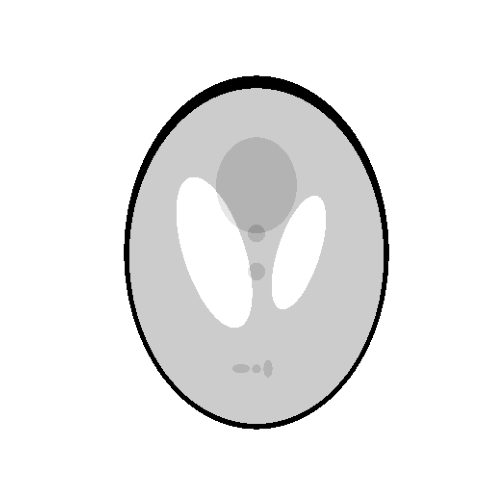
\includegraphics[width=0.3\textwidth]{phantom.png}}
    \hfill
    \subbottom[\label{fig:phantom_sinogram}]{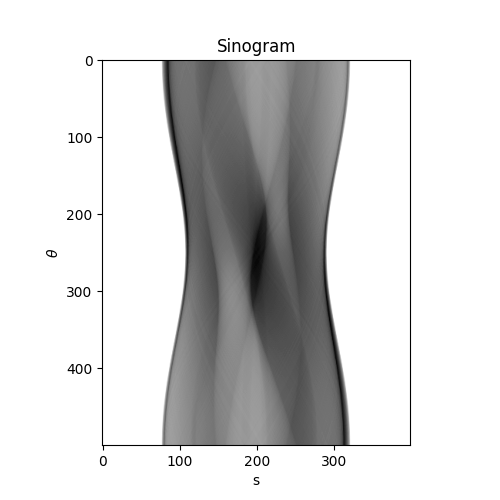
\includegraphics[width=0.3\textwidth]{phantom_sino.png}}
    \hfill
    \subbottom[\label{fig:phantom_sinogram_noisy}]{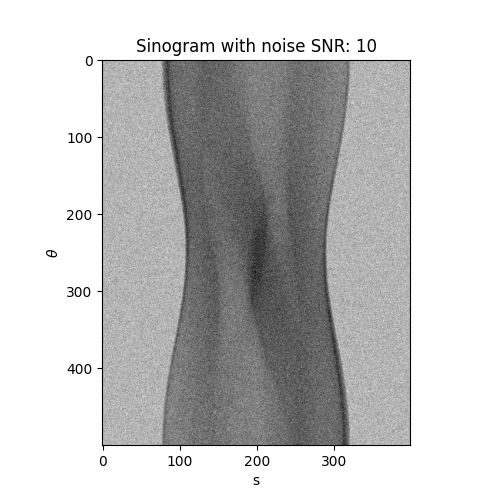
\includegraphics[width=0.3\textwidth]{phantom_sino_noisy_snr10.png}}
    \hfill
	\caption{Shepp-Logan phantom and sinograms: \\
    \ref{fig:phantom} Shepp-Logan phantom: $x$ \\
    \ref{fig:phantom_sinogram} Clean sinogram: $R(x, \theta, s) = p$ \\
    \ref{fig:phantom_sinogram_noisy} Noisy sinogram: $R(x, \theta, s) + \eta = y + \eta$ 
    }
\end{figure}

\subparagraph{Filter Backprojection:}
Filter Backprojection \cite{tomographicReconstruction} (FBP), 
is a reconstruction method, typically used in classical tomography.
It allows to inverse the Radon Transform and enables reconstruction of the original object $x$.
It can be defined as:

\begin{equation}
    \label{eq:fbp}
    \textit{FBP}(\cdot; \theta, s) : L^2(\tilde{\Omega}) \to L^2(\Omega), y \mapsto \textit{FBP}(y; \theta, s)
\end{equation}

with $\theta$ as projection angles and $s$ sampling points. 
The algorithm fails when working with noisy data~\cite{cryoEmMath2}, as it is not possible anymore to draw meaningful connections.

\begin{figure}[h]
    \label{fig:phantom_fbps}
    % \centering
    \hfill
    \subbottom[\label{fig:fbp_phantom}]{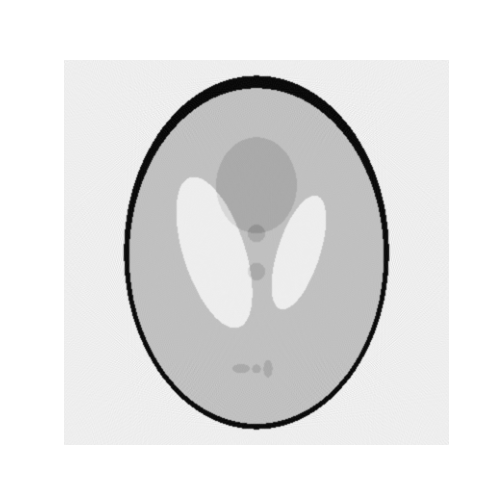
\includegraphics[width=0.3\textwidth]{fbp_phantom_clean.png}}
    \hfill
    \subbottom[\label{fig:fbp_phantom_noisy}]{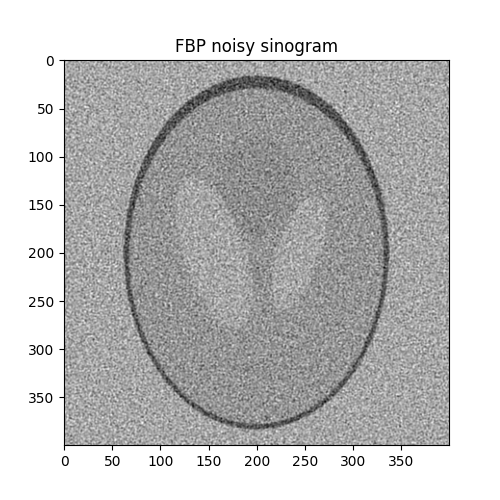
\includegraphics[width=0.3\textwidth]{fbp_phantom_snr_10.png}}
    \hfill
    \subbottom[\label{fig:fbp_unet_phantom_noisy}]{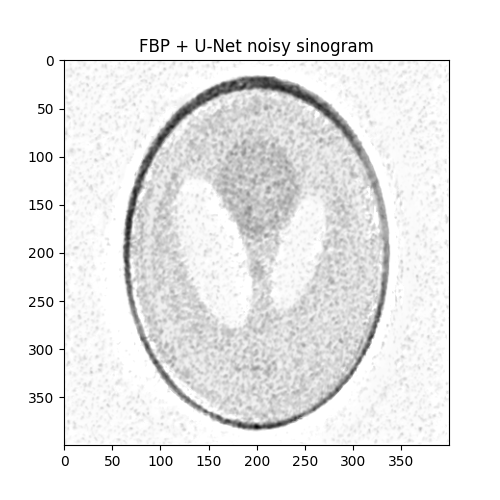
\includegraphics[width=0.3\textwidth]{fbp_unet_phantom_snr_10.png}}
    \hfill
	\caption{Shepp-Logan FBP reconstructions: \\
    \ref{fig:fbp_phantom} Clean reconstruction: $\textit{FBP}(p, \theta, s)$  \\
    \ref{fig:fbp_phantom_noisy} Noisy reconstruction: $\textit{FBP}(y, \theta, s)$ \\
    \ref{fig:fbp_unet_phantom_noisy} Noisy reconstruction: $\textit{UNet}(\textit{FBP}(y, \theta, s))$ 
    }
\end{figure}

In Figure~\ref{fig:fbp_phantom} and Figure~\ref{fig:fbp_phantom_noisy} reconstruction can be seen from 
Shepp-Logan phantom sinogram (figure~\ref{fig:phantom_sinogram}) and its noisy version (figure~\ref{fig:phantom_sinogram_noisy}).
The quality of noisy reconstruction is rather low, some important details are missing, and the noise dominates reconstruction.
If more noise is present in $y$, reconstruction will be of even lower quality.

\subparagraph{U-Net}
\citet{ct-reconstruction-comparison} compared different reconstruction methods for computed tomography. 
Today's state-of-the-art reconstruction algorithms are Deep-Learning based.
U-Net~\cite{unet-tomography}, a convolution neural network approach, performed
much better than only applying FBP, especially when dealing with noise.

During practical part of the Thesis, U-Net was used and trained on lodopab-ct dataset~\cite{lodopab-dataset}, a brain CT dataset. 
More details on U-Net and how it was used can be found in 
Chapter~\ref{sec:contribution} \textit{\nameref{sec:contribution}} and 
Chapter~\ref{sec:results} \textit{\nameref{sec:results}}.
In Figure~\ref{fig:fbp_unet_phantom_noisy}, reconstruction using FBP and U-Net can be seen.
Quality of reconstruction is still not perfect, but overall noise is drastically decreased.


\section{Cryo-EM}
Cryo-EM is another molecular imaging method, that enables the view of molecules in near-atomic resolution.
In this Master's Thesis, for simplicity, only single-particle cryo-EM \cite{singleParticleCryoEm} is considered, 
when writing about cryo-EM it always refers to single-particle cryo-EM.

During imaging process molecules are frozen in a thin layer of ice, where they are randomly oriented and positioned. 
Random orientation and positioning makes reconstruction challenging, 
but freezing allows observation in a stable state where molecules are not moving.
With an electron microscope, two-dimensional tomographic projection images of molecules in the ice are observed,
which are called \textit{micrograph}. 
Frozen molecules are fragile, and electron microscope needs to work with
very low power (electron dose), resulting in highly noisy images. The resulting (SNR)
is typically smaller than 1, which indicates that there is more noise than signal \cite{cryoEmMath2}.

Further, observed molecules are not equal in the sense that there are some structural varieties between
molecules (isotopes). While observing same molecule in ice many times, single observation could be from different isotopes.

\paragraph{3D cryo-EM reconstruction:}
Similar to tomographic reconstruction, cryo-EM reconstruction problem \cite{cryoEmMath} is defined.
It can be seen as a 3D problem as the original object $x \in L^2(\Omega)$ to be reconstructed is in 3D.
Based on many observed micrographs, collected by the electron microscope, original object $x$ will be estimated.

Cryo-EM reconstruction is computational intensive and multiple steps are needed to get from observed
raw data to the final structure (for further details \cite{singleParticleCryoEm} can be consulted).


\paragraph{3D cryo-EM observation:}
Mathematically, observation is defined as follows:
\begin{equation}
    \label{eq:cryoEmSimple}
    \begin{aligned}
        y_i &= p_i + \eta_i, \text{ with } 1 \leq i \leq N,\\
        y_i &= \Pi_z  (\; Rot (\;x; \theta_i )) + \eta_i, \text{ with } 1 \leq i \leq N,    
    \end{aligned}
\end{equation}

where 
\begin{itemize}
    \item $N$: number of observations
    \item $M$: observation dimension
    \item $y_i \in \mathbb{R}^M$:  $i$-th observation with $y_i[j] \in \mathbb{R}$: $j$-th element of observation
    \item $p_i \in \mathbb{R}^M$:  $i$-th noiseless observation with $p_i[j] \in \mathbb{R}$: $j$-th element of observation
    \item $x \in L^2(\Omega)$: original object with $\Omega \subset \mathbb{R}^3 $ and $L^2$: Lebesgue space
    \item $\Pi_z : L^2(\Omega) \to L^2(\tilde{\Omega}), x \mapsto  \int x(\cdot,\cdot,z) dz$: Z-axis projection operator,
          with $\tilde{\Omega} \subset \mathbb{R}^2$
    \item $\theta_i = [\theta_i^{(1)}, \theta_i^{(2)}, \theta_i^{(3)} ] $: 3D rotation matrix with $ \theta_i^{(1)}, \theta_i^{(2)}, \theta_i^{(3)} \in \mathbb{R}$ and \\
          $R_{\theta_i} =  R_{e_x} (\theta_i^{(1)}) R_{e_y} (\theta_i^{(2)}) R_{e_z} (\theta_i^{(3)}) = [R^1_{\theta_i}, R^2_{\theta_i}, R^3_{\theta_i}] \in SO(3)$ \\
          (see \ref{app:3DrotationMatrix} for further details)
    \item $\textit{Rot} : L^2(\Omega) \to L^2(\Omega), \textit{Rot}(x, \theta_i) = \left((x_1,x_2,x_3) \mapsto x( x_1R^1_{\theta_i}, x_2R^2_{\theta_i}, x_3R^3_{\theta_i})\right)$: rotation operator
    \item $\eta_i \in \mathbb{R}^M$: Gaussian noise with $\eta_i[j] \sim \mathcal{N}(0,\sigma^2) \in \mathbb{R}$
\end{itemize}

% $y_i \in \mathbb{R}^M$ with $M$ as observation dimension.

% Then, $\Pi_z : L^2(\Omega) \to L^2(\tilde{\Omega}), x \mapsto  \int x(\cdot,\cdot,z) dz$ is projection operator from z-axis
% and $Rot : L^2(\Omega) \to L^2(\Omega), Rot(x, \theta_i) = \left((x_1,x_2,x_3) \mapsto x( x_1R^1_{\theta_i}, x_2R^2_{\theta_i}, x_3R^3_{\theta_i})\right)$ is rotation operator modelling the rotation during freezing.
% Further, $\theta_i = [\theta_i^{(1)}, \theta_i^{(2)}, \theta_i^{(3)} ] $ where entries $ \theta_i^{(1)}, \theta_i^{(2)}, \theta_i^{(3)} \in \mathbb{R}$ and 
% $R_{\theta_i} =  R_{e_x} (\theta_i^{(1)}) R_{e_y} (\theta_i^{(2)}) R_{e_z} (\theta_i^{(3)}) = [R^1_{\theta_i}, R^2_{\theta_i}, R^3_{\theta_i}] \in SO(3)$ is the 3D rotation matrix 
% (see \ref{app:3DrotationMatrix} for further details). 
% $\eta_i \sim \mathcal{N}(0,\sigma^2I) \in \mathbb{R}^M$ corresponds to noise of observation.


As $y_i$ is not observable directly, discretization is needed:
\begin{equation}
    \label{eq:cryoEmSimpleDiscrete}
    \begin{aligned}
        y_i &= \left( \Pi_z (\; Rot (\;x; \theta_i)) + \eta_i\right)(\Delta), \text{ with } 1 \leq i \leq N \\
        y_i[j,k] &= \Pi_z (\; Rot(\;x; \theta_i))_{j,k} + \eta_i[j,k], \text{ with } 1 \leq i \leq N \text{ and } 1 \leq j,k \leq M,
    \end{aligned}
\end{equation}

where 
\begin{itemize}
    \item $\Delta \subset \tilde{\Omega}^{M^2}$: sampling grid with dimension $M^2$
    \item Further, $y[j,k]$, $\eta[j,k]$ and $\Pi_z(\cdot)_{j,k}$ $ \in \mathbb{R}$ with $j,k$ as indices of the sampling grid.
\end{itemize}
% $\Delta \subset \tilde{\Omega}^{M^2}$ is the sampling grid with dimension $M^2$.
% Further, $y[j,k]$, $\eta[j,k]$ and $\Pi_z(\cdot)_{j,k}$ $ \in \mathbb{R}$ with $j,k$ as indices of 
% the sampling grid.


\begin{figure}[H]
    \label{fig:cryo-em-omicron}
    % \centering
    \hfill
    \subbottom[\label{fig:omicron}]{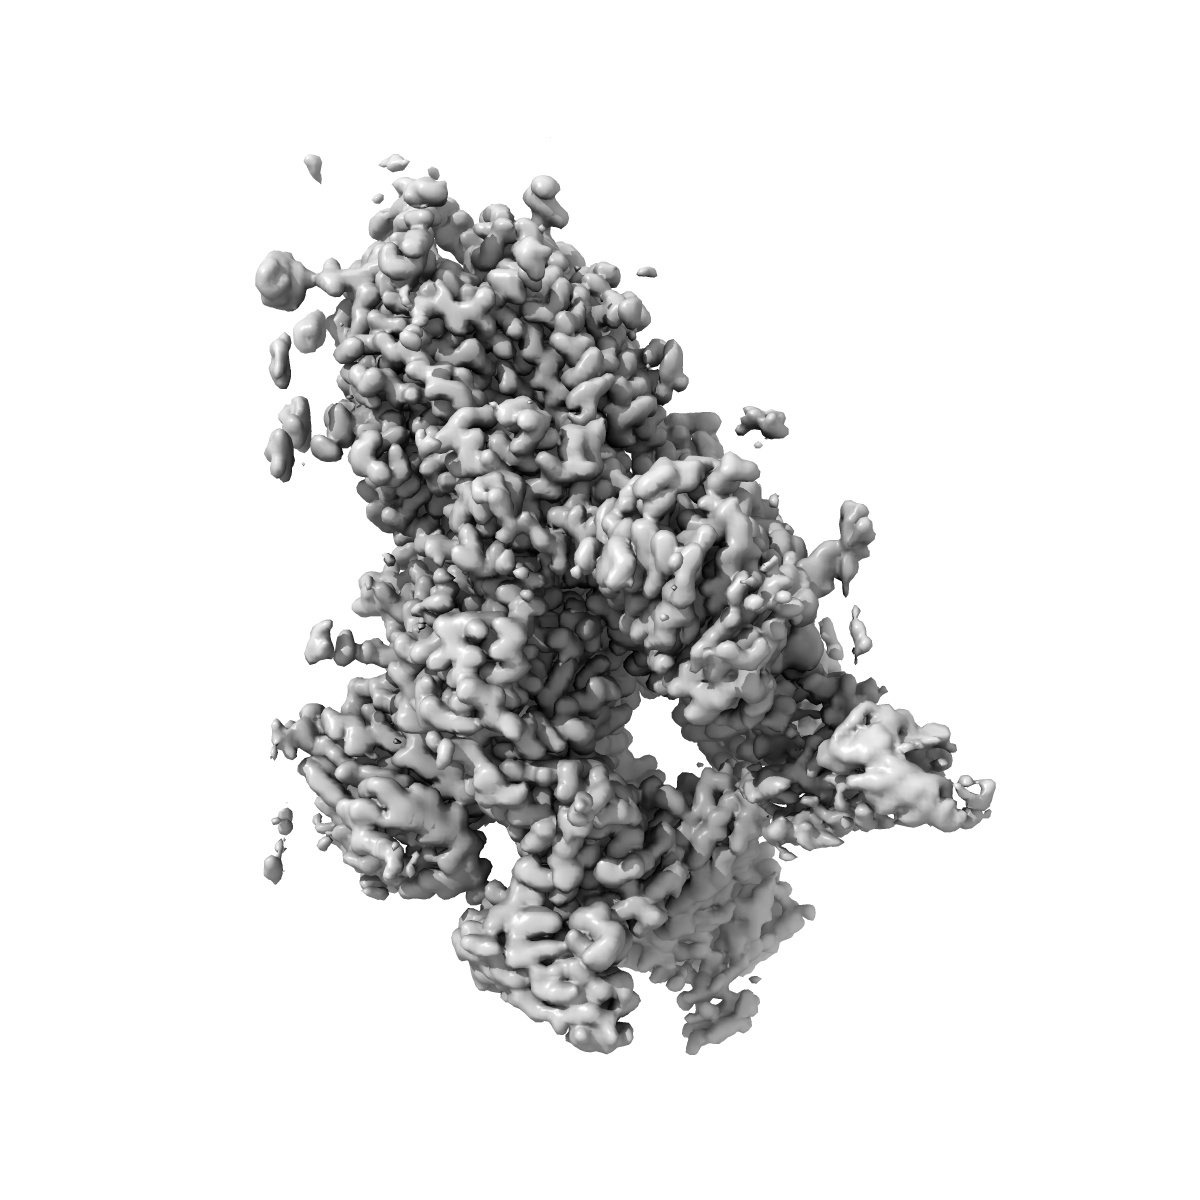
\includegraphics[width=0.18\textwidth]{emd_32500.map_xsurface.jpeg}}
    \hfill
    \subbottom[\label{fig:omicron-x}]{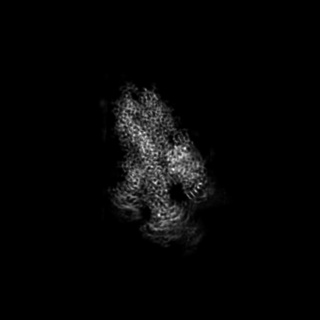
\includegraphics[width=0.18\textwidth]{emd_32500.map_xprojection.jpeg}}
    \hfill
    \subbottom[\label{fig:omicron-y}]{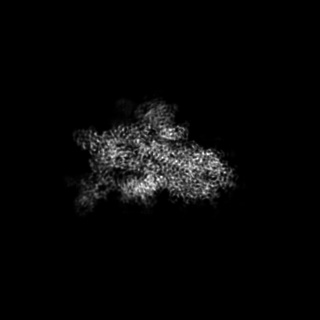
\includegraphics[width=0.18\textwidth]{emd_32500.map_yprojection.jpeg}}
    \hfill
    \subbottom[\label{fig:omicron-z}]{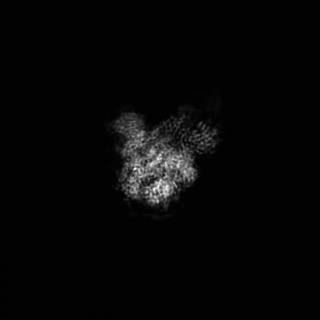
\includegraphics[width=0.18\textwidth]{emd_32500.map_zprojection.jpeg}}
    \hfill
	\caption{Cryo-EM reconstruction and clean projections of COVID-19 Omicron spike \protect\footnote{https://www.ebi.ac.uk/emdb/EMD-32500}: \\
    \ref{fig:omicron} COVID-19 Omicron spike: $x$ \\
    \ref{fig:omicron-x} projection along x-axis: $p_1$ \\
    \ref{fig:omicron-y} projection along y-axis: $p_2$  \\
    \ref{fig:omicron-z} projection along z-axis: $p_3$ \\
    }
\end{figure}


\subparagraph{Extended formula:} 
Equation~\ref{eq:cryoEmSimple} is a simplified version of cryo-EM.
First, point spread function (PSF) of the microscope is not taken into account.
Secondly, structural variety is ignored, the underlying object $x$ is not the same 
for every observation as modelled in the Equation. 
Precisely, $x$ can be seen as a random signal from an unknown distribution defined over all possible molecules structures.

Equation can be extended and defined as the following:
\begin{equation}
    \label{eq:cryoEmExtended}
    y_i = h_i \circ \Pi_z ( \textit{Rot} (x_i; \theta_i)) + \eta_i, \text{ with } 1 \leq i \leq N
\end{equation}

where $h_i$ is the PSF of the microscope and $\circ$ defines the convolution.
Further, $x_i \in X$ where $X$ is the set of all possible molecule structures.


\subparagraph{Difference to tomographic reconstruction:}
The problems are highly related, but cryo-EM reconstruct is more challenging.
While CT observation, patient is asked to not move and therefore, angles of projections are known.
Whereas, in cryo-EM, this information will be lost during freezing.
Secondly, high level of noise makes cryo-EM much more challenging.

\clearpage

\section{Abstraction}

\label{sec:abstract_form}
As tomographic reconstruction and cryo-EM reconstruction are rather similar, 
goal of this Thesis will be to design an algorithm, that can be applied in both scenarios.

Therefore, an abstract form of the problems will be defined.
A similar notation than previously is used, with original object $x \in L^2(\Omega)$.
Further, original object dimension space is parametrized with $D$, consequently $\Omega \subset \mathbb{R}^D$.
Additionally, dimension of observation space is defined as $D-1$, such that 
$\tilde{\Omega} \subset \mathbb{R}^{D-1}$.


\begin{equation}
    \label{eq:abstract-model}
    \begin{aligned}
        y_i &= p_i + \eta_i (\Delta), \text{ with } 1 \leq i \leq N \\
        y_i &= \left( A(x, \theta_i) + \eta_i \right) (\Delta), \text{ with } 1 \leq i \leq N 
    \end{aligned}
\end{equation}
with
\begin{itemize}
    \item $N$: number of observations
    \item $M$: observation dimension
    \item $y_i \in \tilde{\Omega}^M$: the $i$-th observation
    \item $p_i \in \tilde{\Omega}^M$: the $i$-th noiseless observation
    \item $x \in L^2(\Omega)$: original object
    \item $A: L^2(\Omega) \to L^2(\tilde{\Omega}), x \mapsto A(x; \theta_i)$: a non-linear operator 
    \item $\theta_i \in \mathbb{R}^P$: projection angle vector, with $P$ projection dimension
    \item $\eta \sim \mathcal{N}(O, \sigma^2 I) \in \tilde{\Omega}^M$: Gaussian noise
    \item $\Delta \subset \tilde{\Omega}^{M}$: term for discretization
\end{itemize}

\paragraph{Reconstruction:}
Further, an abstract form of the reconstruction operator is defined as 

\begin{equation}
    \textit{Recon} : L^2(\tilde{\Omega}) \to L^2(\Omega), y \mapsto Recon(y; \theta) (\Delta)
\end{equation}

with
\begin{itemize}
    \item $\theta_i \in \mathbb{R}^P$: projection angle vector, with $P$ projection dimension
    \item $\Delta \subset \tilde{\Omega}^{D}$: term for discretization, $D$ as the dimension of the space of original object
\end{itemize}

\textbf{Check: Theta and discretization term}

\paragraph{Classical tomography:}

Classical tomography parameters are defined with $D=2$, $P=1$.
Further, $A(\cdot)$ is the Radon Transform (see Equation~\ref{eq:2Dreconstruction}).
Reconstruction operator can be defined as FBP (with or without U-Net\cite{unet-tomography}).

\paragraph{Cryo-EM:}
Cryo-EM parameters are defined with $D=3$ and $P=3$ as $\theta_i$ not only corresponds to
a projection angle vector but also some rotation.
Further, $A(\cdot)$ can be defined as $\Pi_z \left(\; \textit{Rot}(\;x; \theta) \right)$ 
where \textit{Rot} is the 3D rotation and $\Pi_z$ the tomographic projection.

\paragraph{High noise regime:}
Cryo-EM observations are highly noisy, which makes reconstruction challenging. 
There are different ways to reduce noise from observations, most of them are related to averaging. 
Averaging needs to consider similar observations and ignore diverse ones. 
In the defined abstract model, averaging over paired observations from $\theta$ should be a good averaging model.
But how can it be achieved? 

One idea would be to measure distances between observation.
Another way is to find a low-dimensional embedding which maps our observations $y$ to some $\theta$.
When talking from low-dimensional embeddings, there is no way around Graph Learning, which will be introduced
in the following Chapter~\ref{sec:graphFoundations} \textit{\nameref{sec:graphFoundations}}.
